\section{System Design}
\label{sec:system}
\subsection{System Overview}
\begin{figure*}[h]
	\centering
	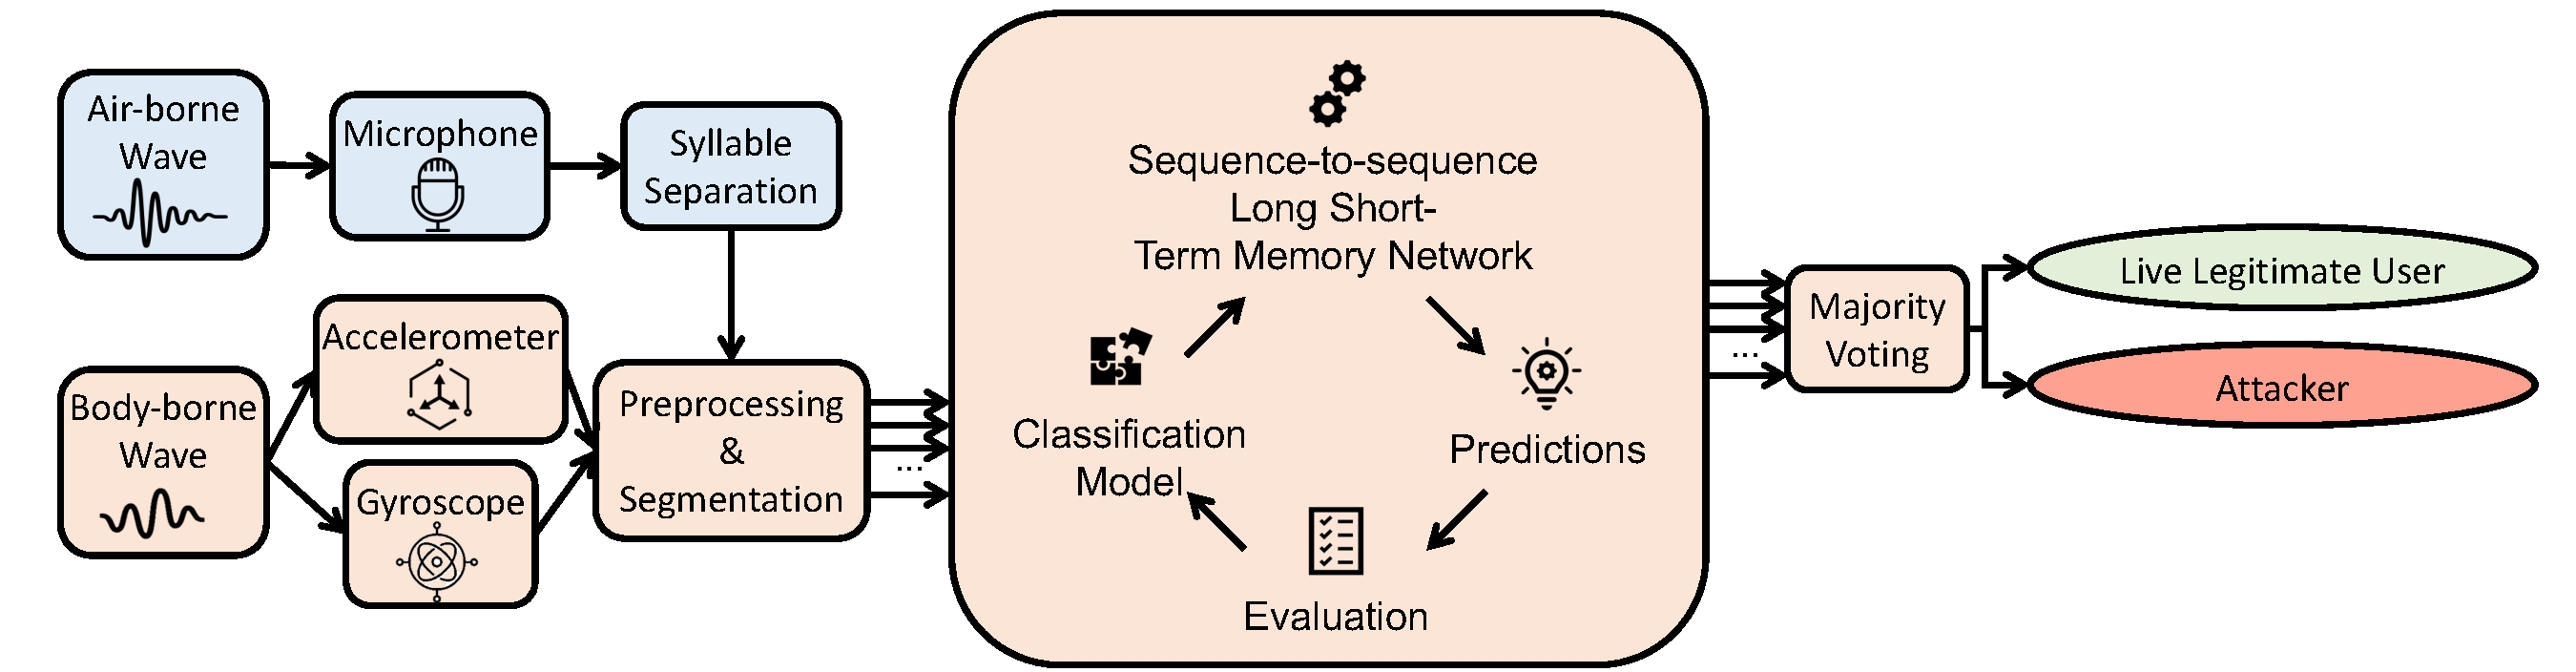
\includegraphics[width=\linewidth]{workflow}
	\caption{The flow of {\shortname}.}
	\label{fig:workflow}
\end{figure*}
\shortname~ currently is a text-dependent voice authentication system. In other words, the speaker recognition algorithm will work on hot-words such as ``Ok Google'', ``Hi Siri'', or ``Alexa''. When a user triggers the voice authentication system, the microphone works normally and the motion sensors measure the modulated and attenuated sound signals at the same time.


Since the hot-words are usually short, less than 2 seconds in our experiment, it is acceptable to process the data together after the whole hot-word is spoken.

We first conduct the syllable separation on speech signals. For example, ``Ok Google'' has 4 syllables in total: O-K-Goo-Gle, ``Hi Siri'' has 3, and ``Alexa'' has 3 too. We will, later on, use the detected hot-word beginning and ending time, as well as the syllable nuclei time to segment the accelerometer and gyroscope data.
%
Since the motion data suffer from noises from body movements, heartbeats, and breathings, we must preprocess the motion data. We apply a high pass filter to mitigate the noises and increase the target signal. 



We then segment the motion data based on different syllables. We focus on data collected among the syllable nucleus. Because when the sound signal is the maximum, the chance is high that the motion is also the maximum. The maximum motion indicates a higher accuracy of the collected data, which is beneficial for training a more effective and efficient classification model.
%
Another benefit of the segmentation is that segmentation provides the opportunity to do majority voting. For the motion data corresponding to ``Ok, Google'', as long as more than half of the samples are classified into the correct category, we regard the speech and throat movement as matching each other. This greatly increases the true positive rate of our liveness detection algorithm.

Due to the low sampling rate of motion sensors, the on-body vibration of speech cannot be fully recorded in motion sensors. Finding good representative features is hard. Therefore, we adopt the long short-term memory (LSTM) network, a variant of the recurrent neural network (RNN), to help us learn the features on time-domain and classify each segment to each syllable. 

After the majority voting on the classification results on all data samples, \shortname~outputs whether the motion data match the live legitimate user's training model. If yes, a live user is asking the permission; otherwise, an attacker is using a speaker to attack the system. 


\begin{figure}[t]
	\centering
	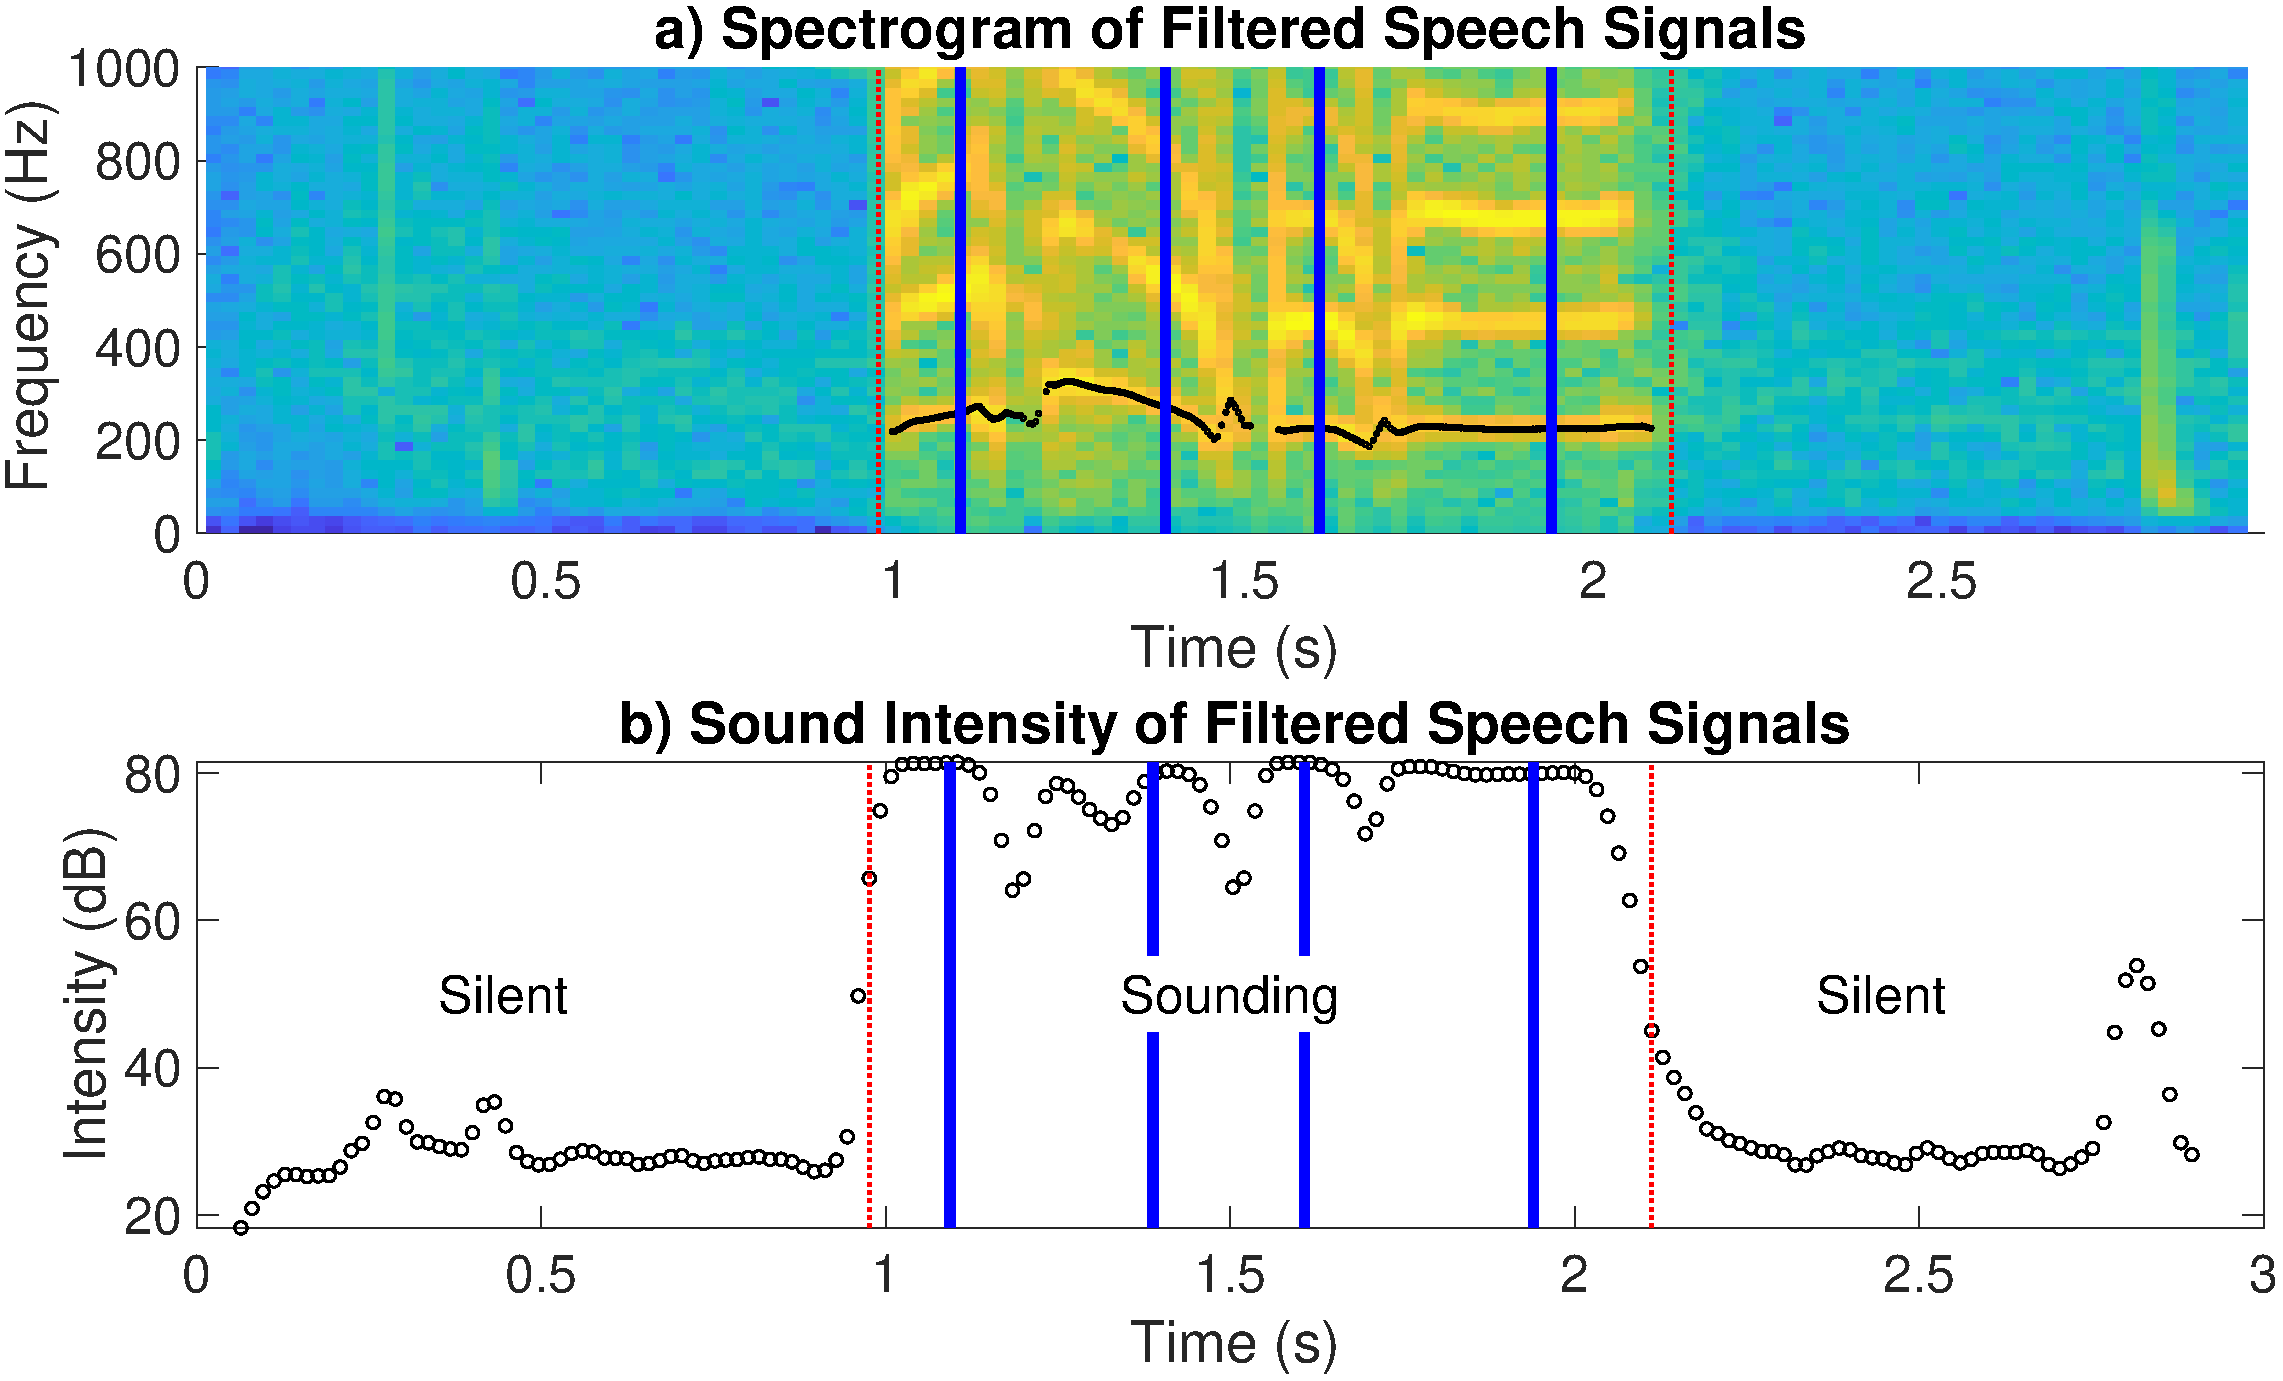
\includegraphics[width=.8\linewidth]{syllable}
	\caption[Syllable Separation]{Syllable Separation. The original signal is a female user saying ``Ok Google''; then the signal is filtered with a bandpass filter with passing frequency range [50 1000]. The black dots in subfigure a) are the calculated pitches. The vertical red dotted lines indicate the start and end of a sounding period. The blue vertical lines show the calculated time for each syllable nucleus.}
	\label{fig:syllable}
\end{figure}
%TODO add arrows

\subsection{Syllable Separation}
A syllable is a unit of pronunciation having one vowel sound, with or without surrounding consonants, forming the whole or a part of a word~\cite{onlinesyllable}. The vowel in the middle of a syllable is referred to as a \textit{nucleus} in phonetics and phonology. We modify the syllable nuclei detection algorithm proposed by De and Wempe~\cite{de2009praat} and the detailed steps are listed as the following:

%, and implement it in the software program Praat~\cite{onlinepraat}.

\textbf{Step 1}. 
Before conducting the syllable separation, we first apply a $\left[50-1000\right]$ Hz bandpass filter to remove noises so that the frequency range is speech-band limited. We then calculate the intensity and pitch to detect the syllable nucleus since the vowel within a syllable has higher energy surrounding sounds. 
%





\textbf{Step 2}. 
The intensity of a sound in air is the sound pressure level relative to $2*10^{-5}$ Pascal, which is the normative auditory threshold for a 1000-Hz sine wave. We calculate the intensity contour by squaring all values in the sound, then convolved with a Kaiser window. To guarantee that a periodic signal is analyzed as having a pitch-synchronous intensity ripple not greater than 0.00001 dB, we set the length of the Kaiser window to be 64 ms and the sidelobe height to be -190 dB. In this way, we are able to find peaks in the energy contour



\textbf{Step 3}. We consider all peaks above a certain threshold
in intensity to be potential syllables. We set the threshold
to 20dB below the maximum intensity measured over the
total sound file.

\textbf{Step 4}. We then use the intensity contour to make sure that the intensity between the current peak and the preceding peak is sufficiently low. We consider only a peak with a preceding dip of at least 2 dB with respect to the current peak as a potential syllable. In this way, we also delete multiple peaks within one syllable.

\textbf{Step 5}.
We use the algorithm proposed by Boersma ~\{boersma1993accurate\} to calculate the pitch (fundamental frequency) contour of audio data. The window size is set to be 100 ms with 20 ms time steps. We then exclude all peaks that are unvoiced. The remaining peaks are considered syllable nuclei and will be used to segment motion data.

Fig.~\ref{fig:syllable} shows the pitch contour in subfigure a) and the intensity contour in subfigure b). The resulting appearance times of syllable nuclei are marked using blue vertical lines.





%\input{preprocess}
\subsection{Preprocessing and Segmentation}
\begin{figure*}[h]
	\centering
	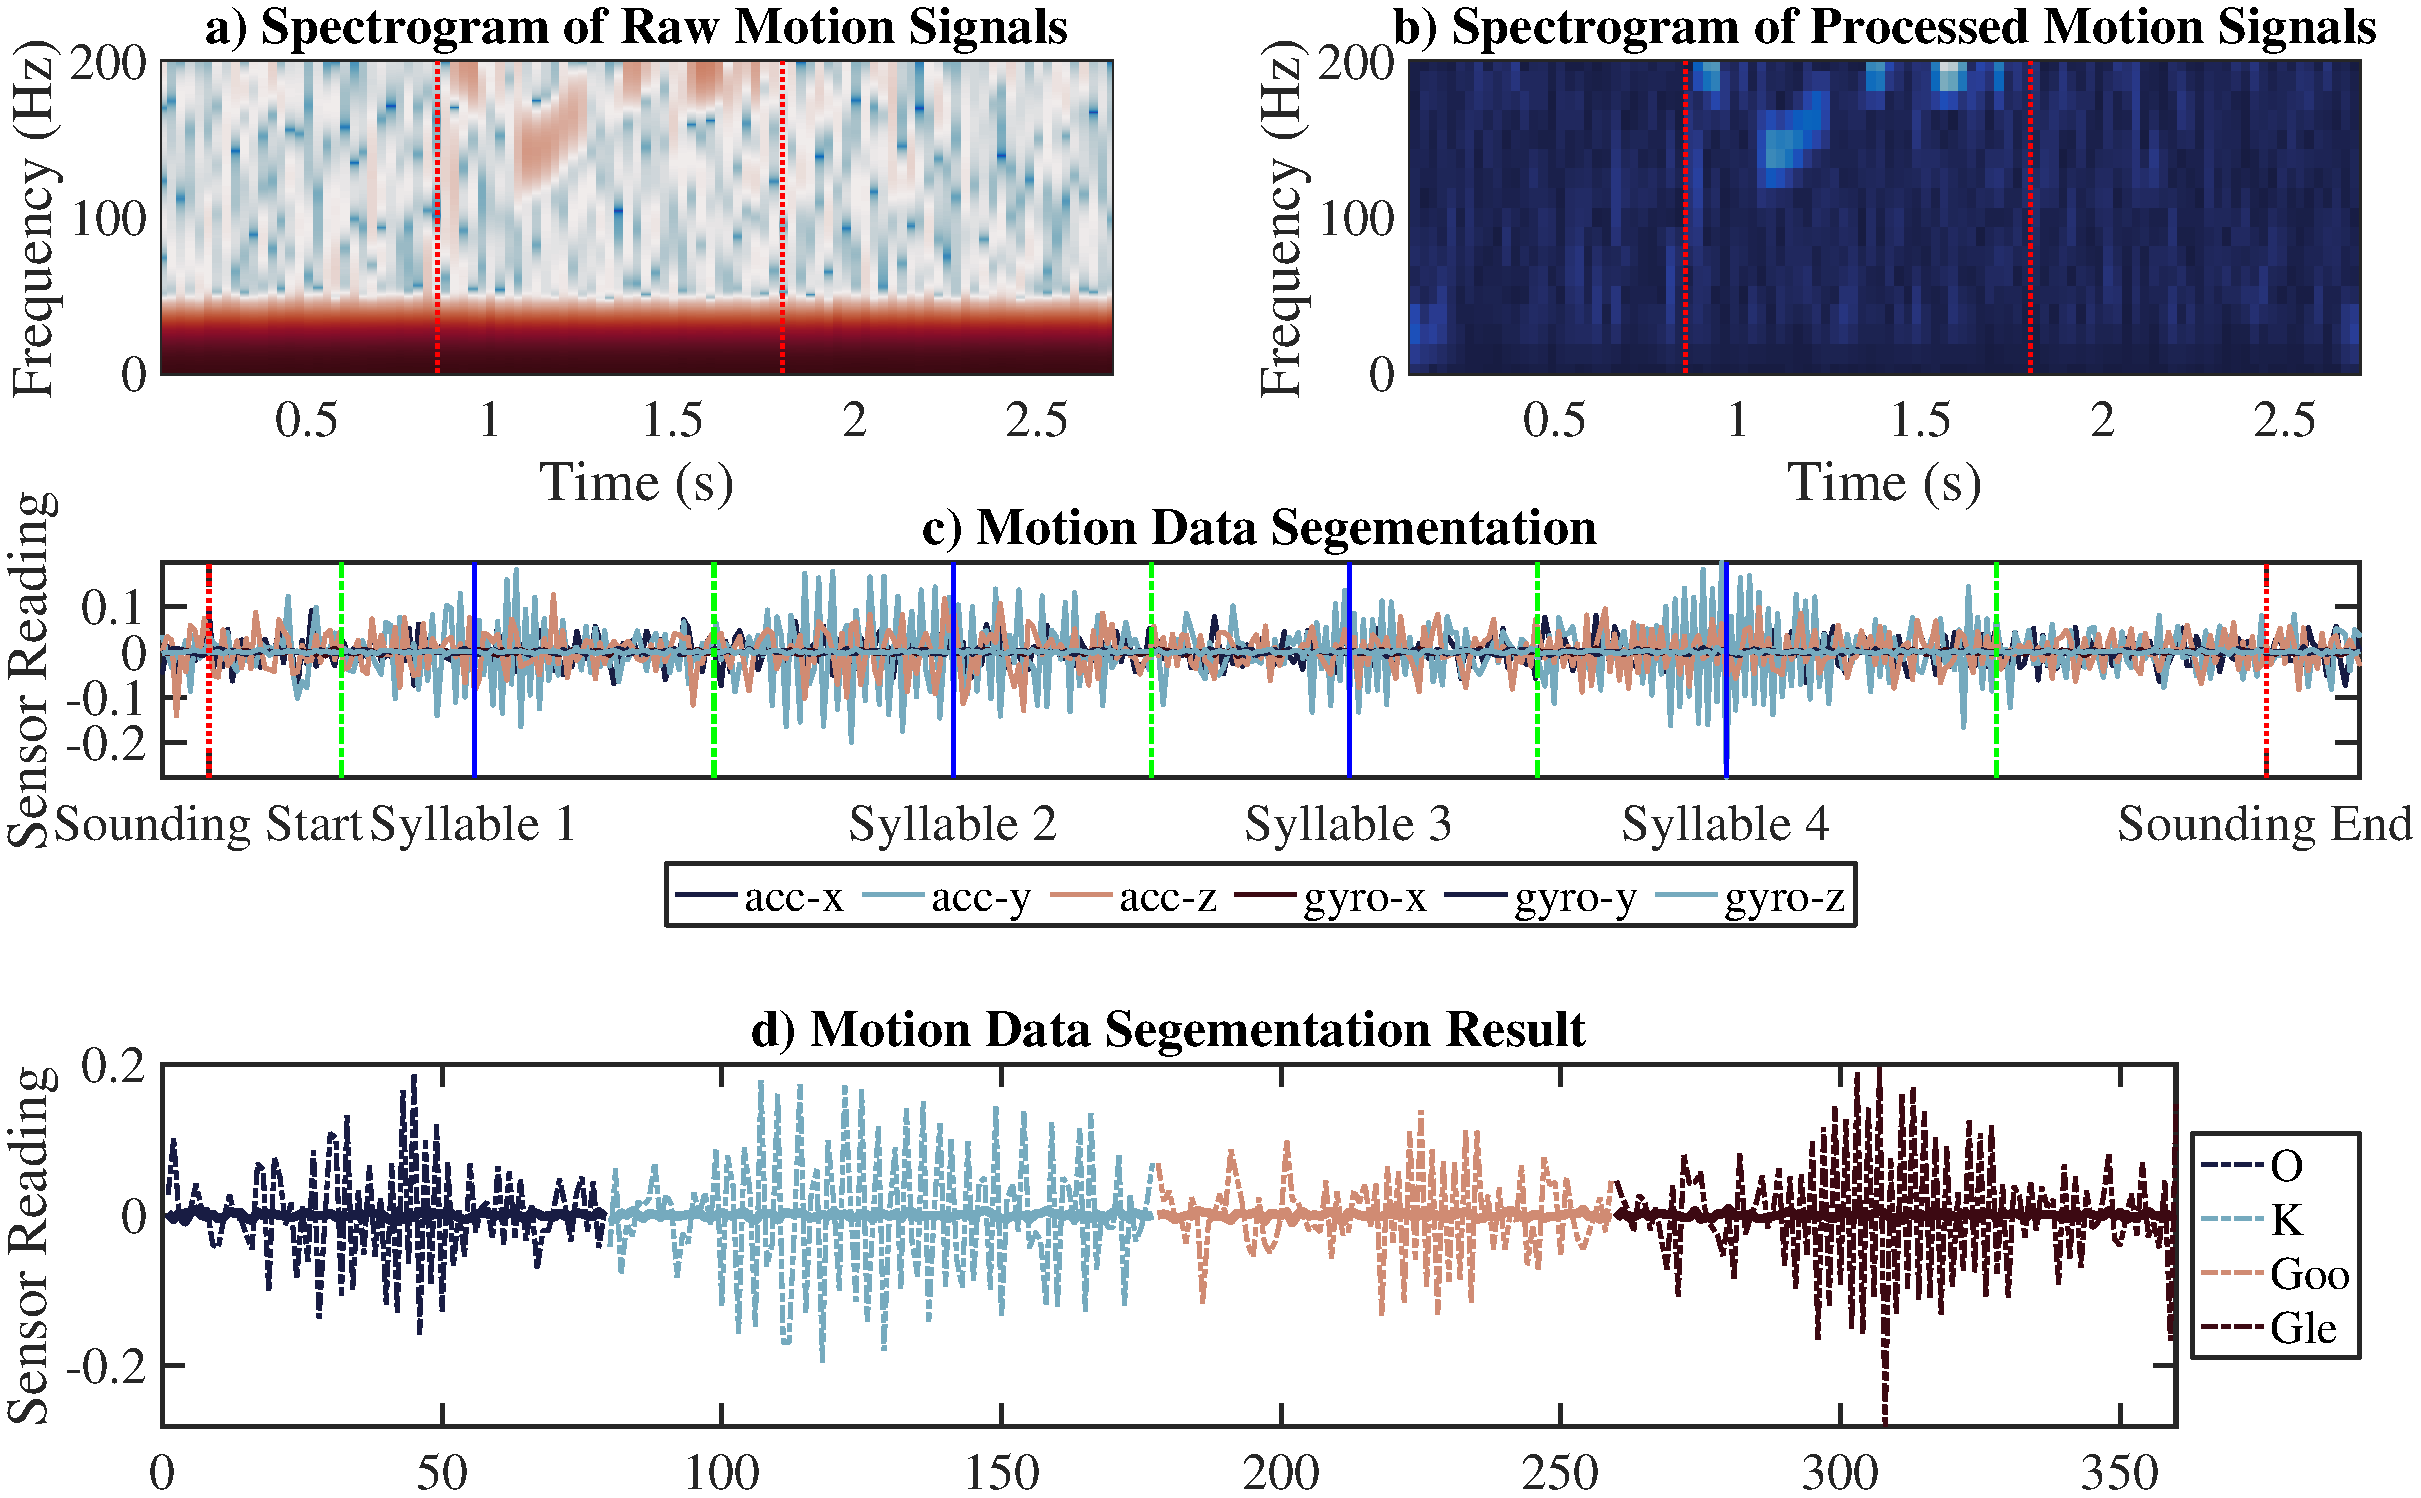
\includegraphics[width=\linewidth]{movopreprocess}
	\caption{Preprocessing and Segmentation. }
	\label{fig:movopreprocess}
\end{figure*}
The motion data is impeded by the low sampling rate, low target movement, and large interference noises. To overcome such a problem, we must preprocess the motion data. We apply a high pass filter to mitigate the noise and increase the signal-to-noise ratio. The cutoff frequency is set to be 100 Hz, since noises such as breathing or walking or other human movements can not create signals as high as 100 Hz. As shown in Fig.~\ref{fig:movopreprocess}, after applying a high pass filter, the motion data in Fig.~\ref{fig:movopreprocess}b is much cleaner than the original data in Fig.~\ref{fig:movopreprocess}a. 

We then use the syllable nuclei calculated in the previous section to segment the motion data. As shown in Fig.~\ref{fig:movopreprocess}c, we first calculate the half time points (green lines) from sounding start time (red line), syllable times (blue lines), and sound end time (red line). Then we extract each segmentation from two adjacent half time points (green lines). Note that if the time duration between two adjacent half time points is large than 100 samples, we will only keep the middle 100-samples data and discard the data at the beginning area and the end area. This is because the data far from syllable nuclei are not as reliable as data around syllable nuclei. Keeping those unreliable data does no good for the classification model.
%
Lastly, concatenating reliable data around syllable nuclei together gives the final processed data. One example of the resulting segmentation is illustrated in Fig.~\ref{fig:movopreprocess}d. Note that Fig.~\ref{fig:movopreprocess}c shows motion data of all six dimensions, while Fig.~\ref{fig:movopreprocess}d only shows two of them: the data of the solid line is from the gyroscope and the data of the dashed line is from the accelerometer.

Note that we do not consider the synchronization problem between the microphone and the motion sensors. This is because the sampling rate of motion sensors is set to be 400Hz, which means that an error with just one sample represents 1/400=0.0025 s. Within such a period of time, the sound travels about 343 m/s * 0.0025 s $\approx$ 0.85 m in air, which is much longer than the distance between the voice source and the microphone. In other words, due to the low sampling rate of motion sensors, the true lag between microphone reading and motion reading always falls in one sample period, which makes the synchronization procedure unnecessary. 

%TODO remove subfigure


%\input{lstm}
\subsection{The LSTM Network}
%TODO RNN
After the preprocessing and segmentation of the motion data, we use the data to establish a sequence-to-sequence Long Short-Term Memory (LSTM) network model. LSTM was first proposed by Sepp Hochreiter and J{\"u}rgen Schmidhuber in 1997 ~\cite{hochreiter1997long}. It is a special variant of Recurrent Neural Networks (RNN), and is widely used in learning, processing, and classifying sequential data because of 
its great property of selectively remembering patterns for long durations of time. Over the years, there have also been many variants of LSTM networks. However, based on a study in 2017, none of the variants can improve upon the standard LSTM architecture significantly~\cite{greff2017lstm}. Therefore, we still choose to implement the standard LSTM network in this work.



Our sequence-to-sequence LSTM has five layers in total and it is able to make different predictions for each individual time step of the input data. In the sequence input layer, the input data have 6 feature dimensions, which consists of 3 accelerometer dimensions and 3 gyroscope dimensions. Then we establish an LSTM layer formed by LSTM blocks, where each block publishes its cell state to the next LSTM block. The output of the LSTM layer is the fully connected hidden status layer. We set the total number of hidden units to be 100, then feed the hidden status to a softmax function and output the classification of each time step of input data.


\section{Majority Voting}

\begin{figure}[t]
	\centering
		\centering
		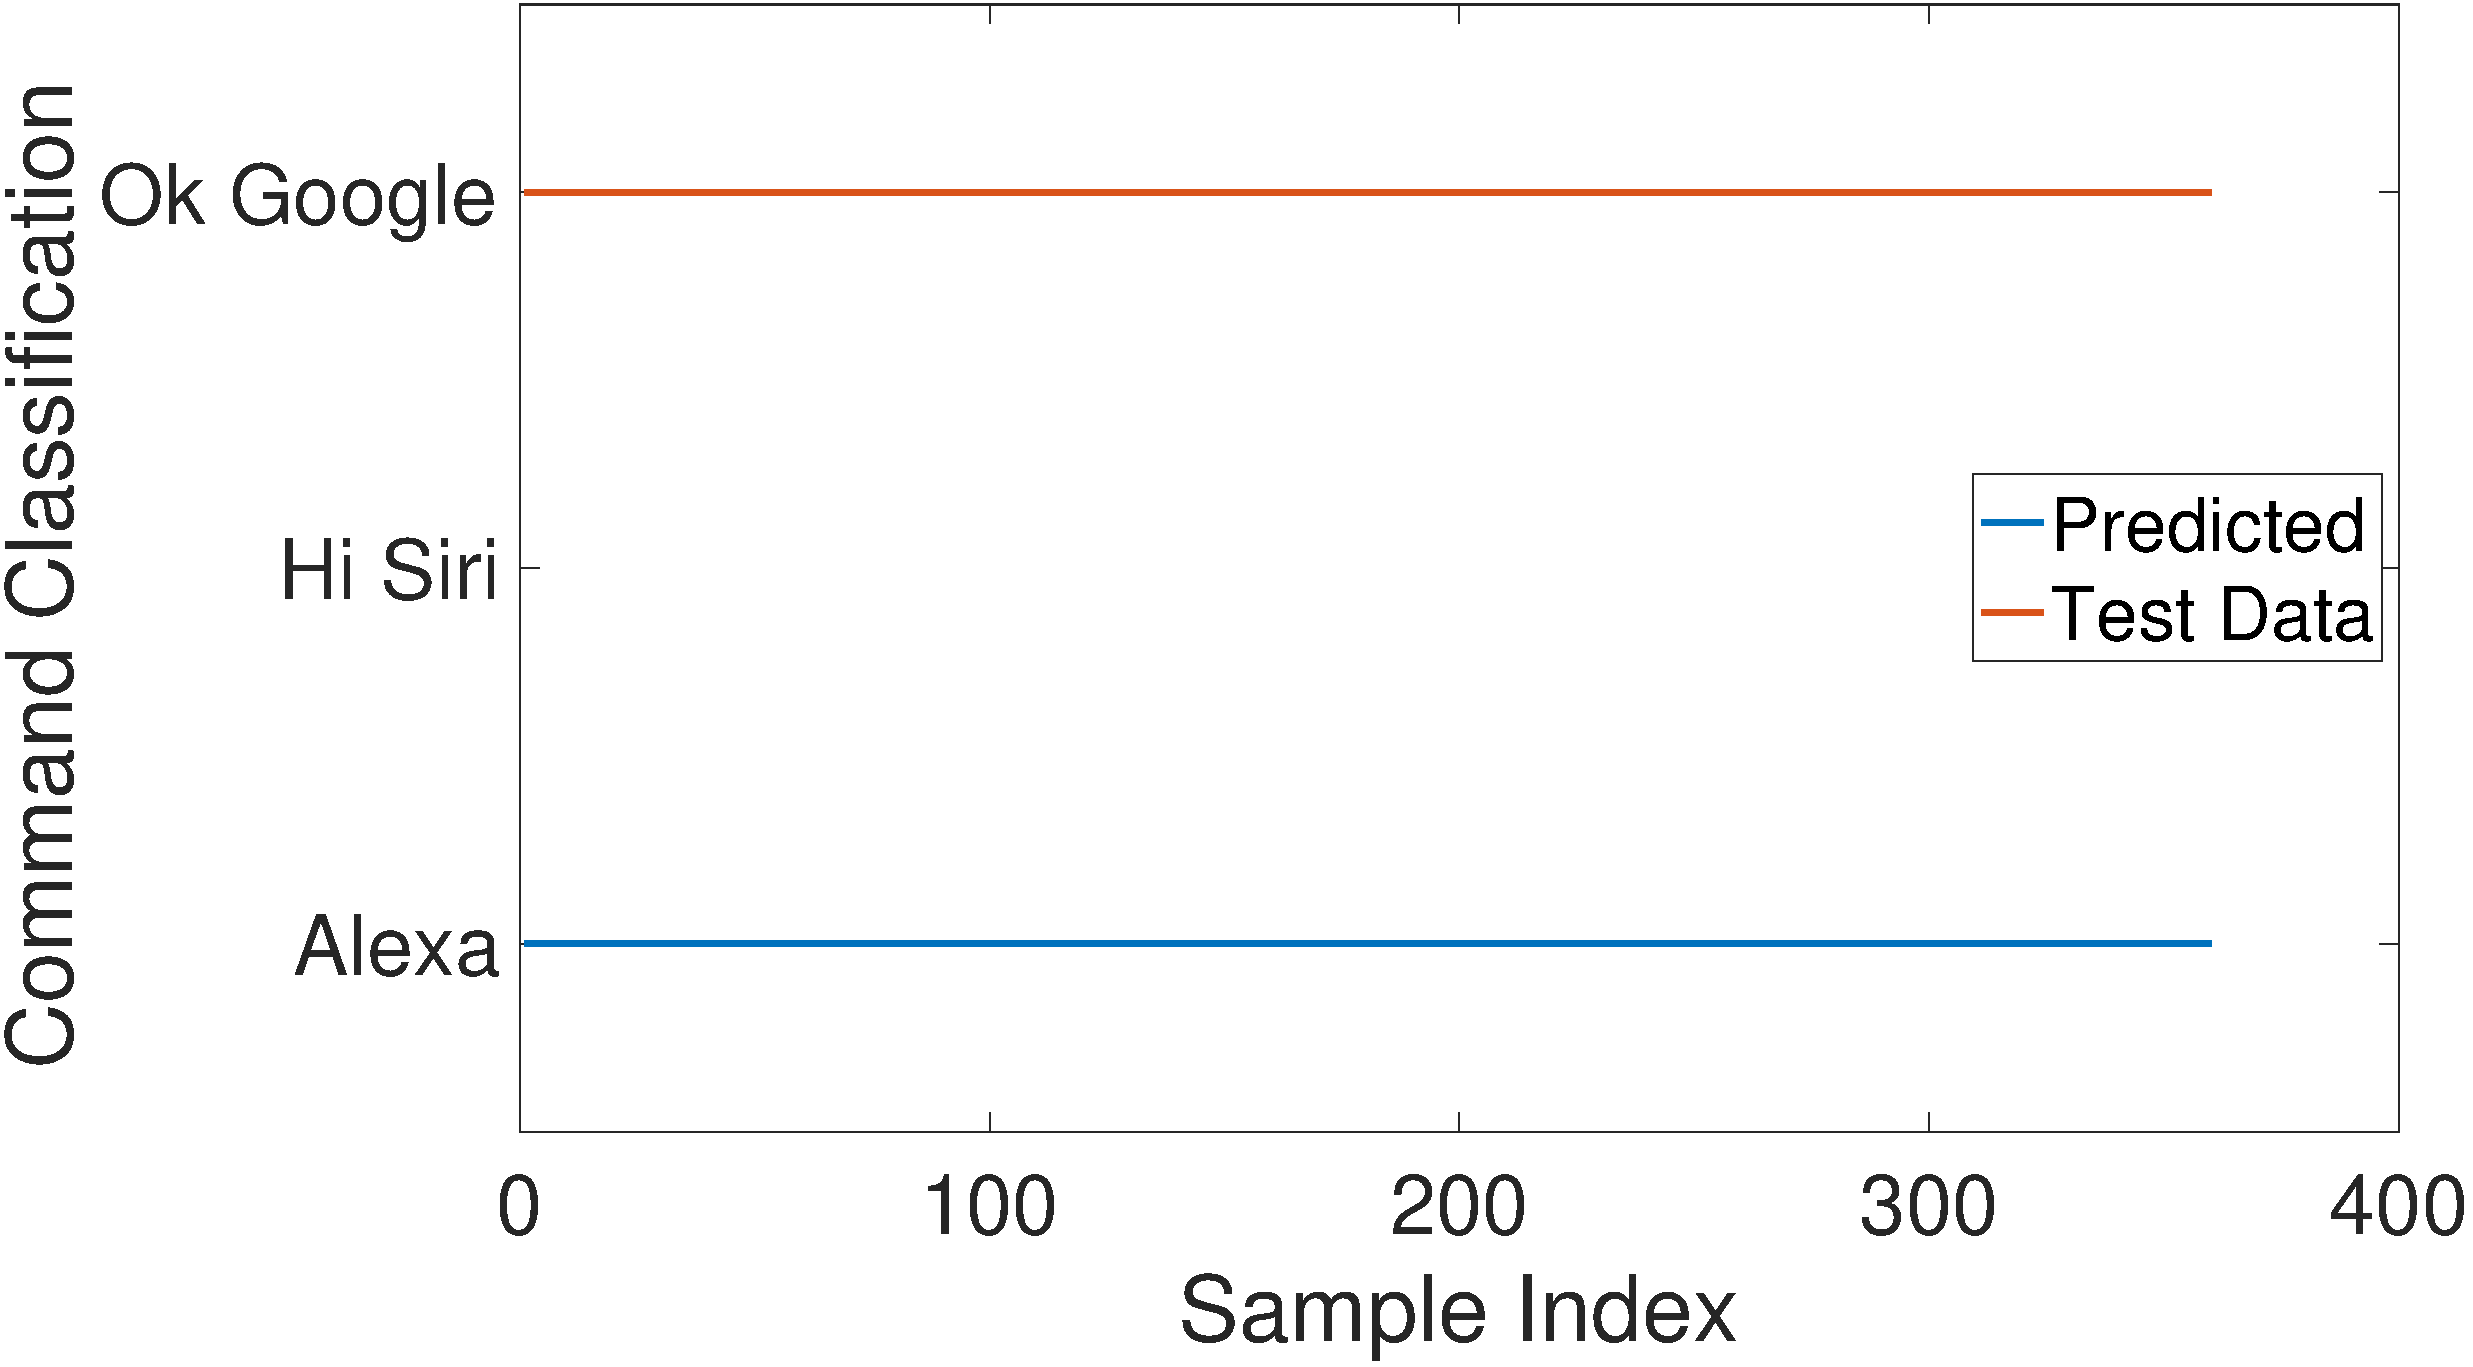
\includegraphics[width=.5\linewidth]{nonmajority}
		\caption{Classification result without syllable separation and majority voting: Falsely classifying an `Ok Google' sample to `Hi Siri'.}
		\label{fig:nonmajority}
\end{figure}
\begin{figure}[t]
		\centering
		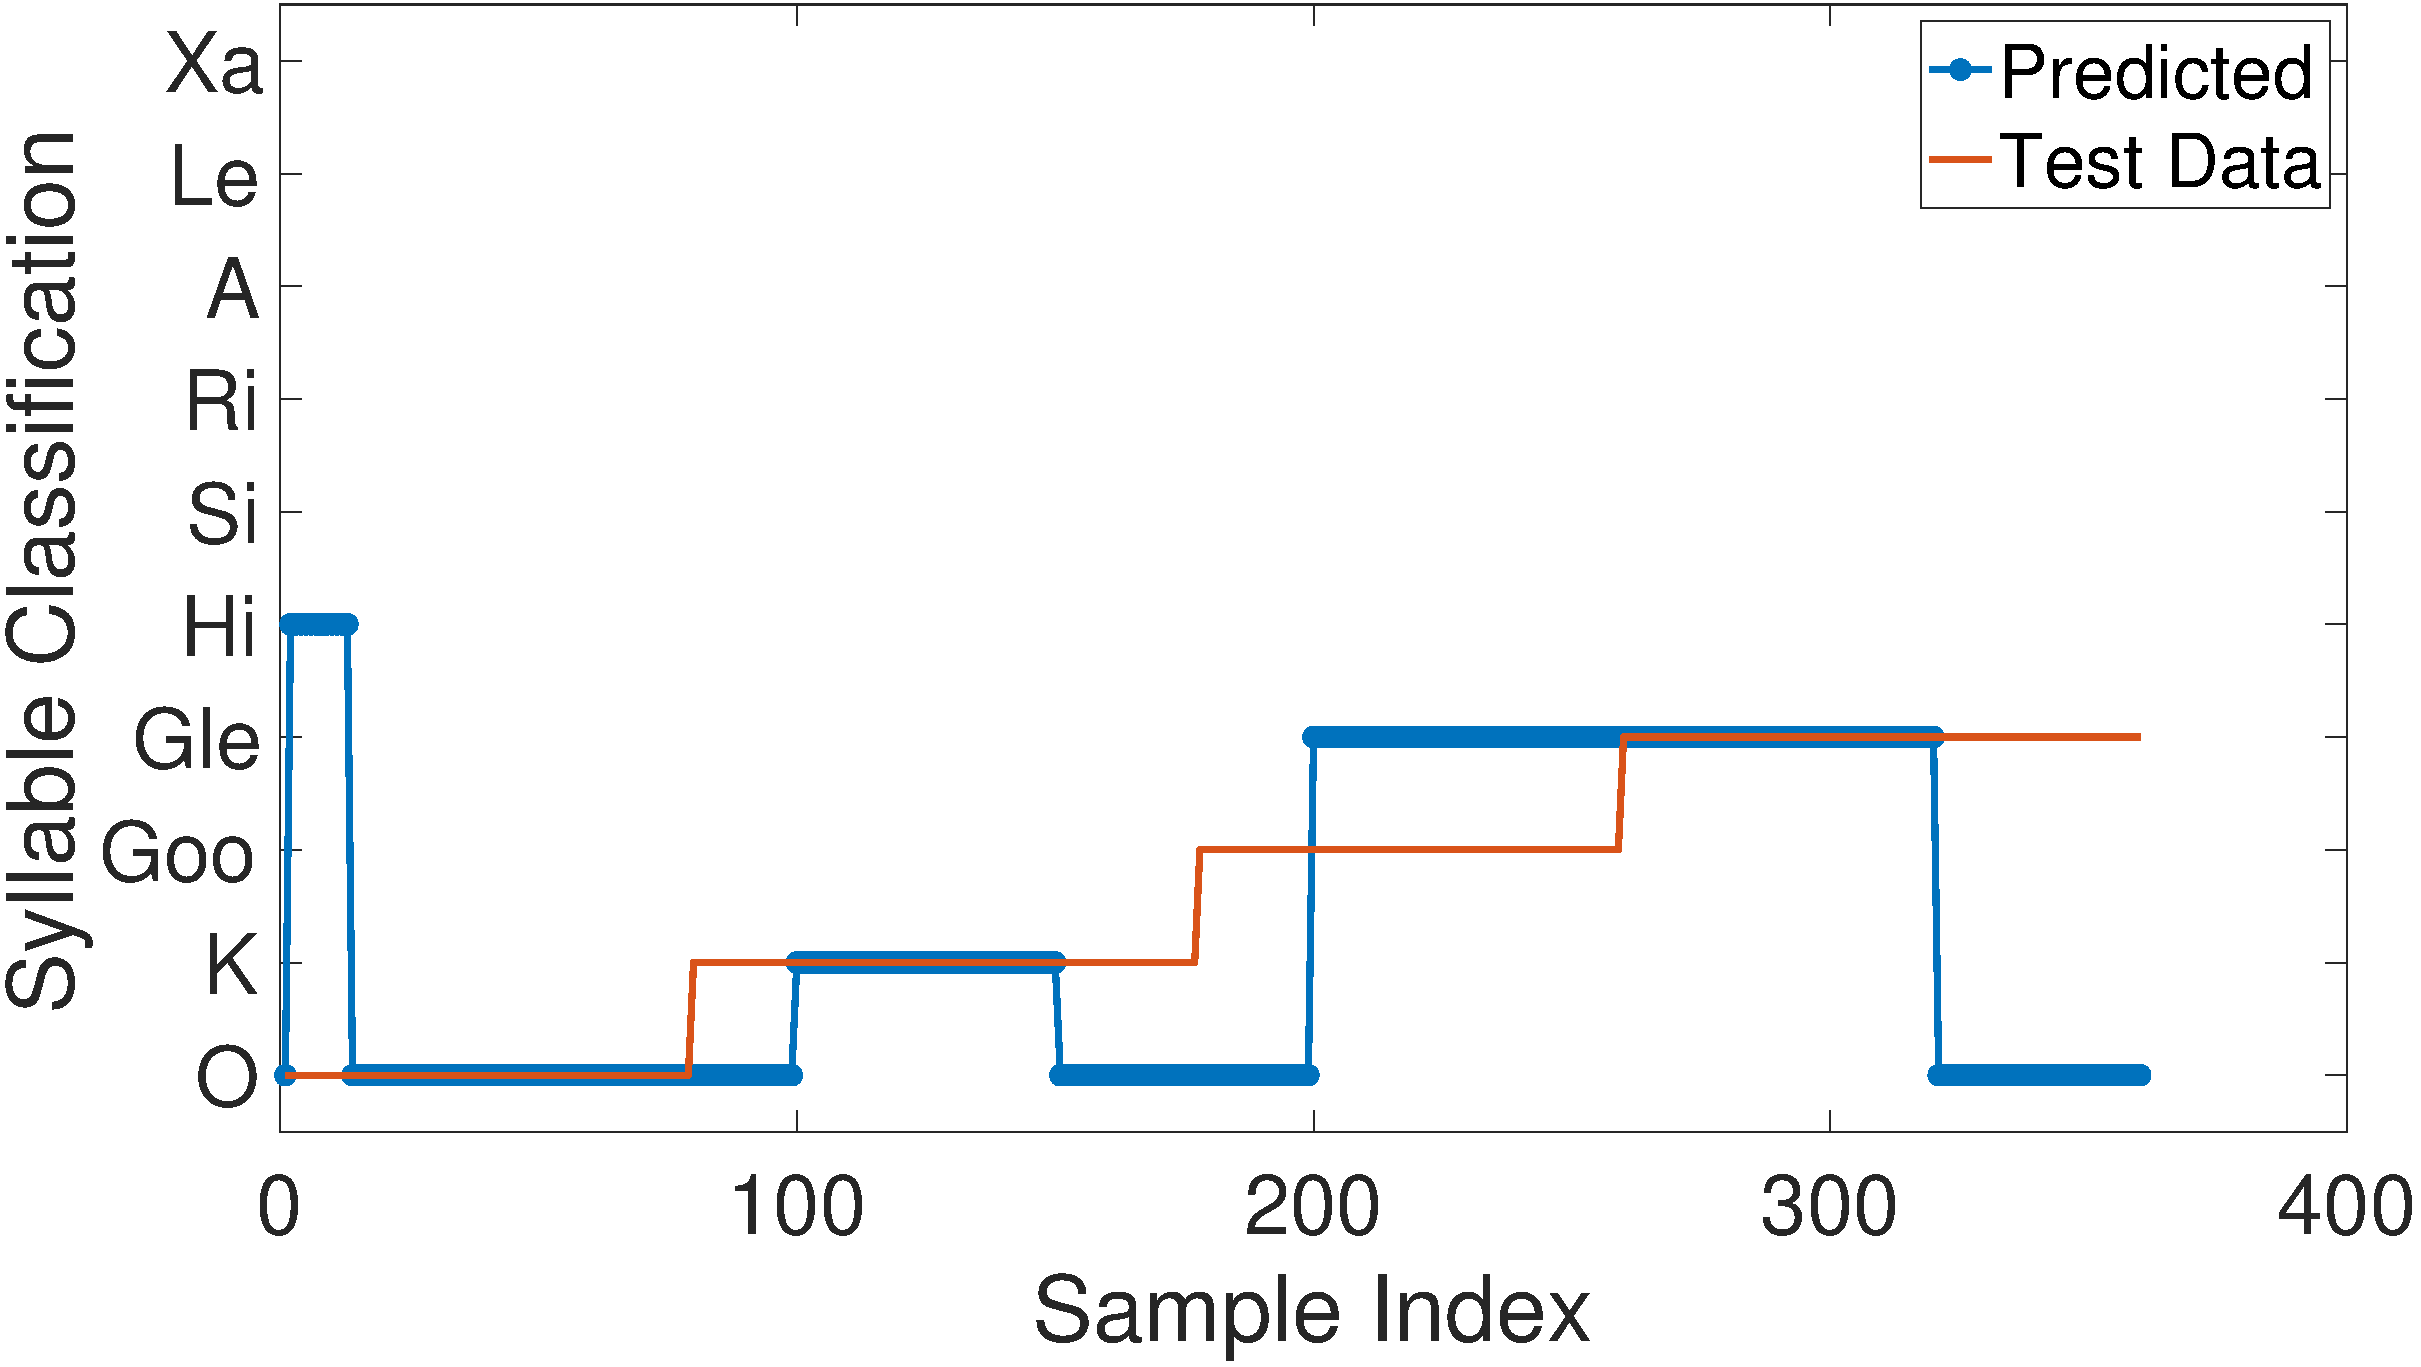
\includegraphics[width=.5\linewidth]{majority}
		\caption[Classification Result]{Classification result from the sequence-to-sequence LSTM network. Although many parts of the classification is incorrect, with majority voting, the final classification is the correct `Ok Google'. }
		\label{fig:majority}
\end{figure}


Since we are using the sequence-to-sequence LSTM network, an example classification result is shown in Fig.~\ref{fig:majority}. Though the ground truth of the test data is O-K-Goo-Gle, the predicted result is O-Hi-O-K-O-Gle-O. However, with a majority voting algorithm, as long as half of the sample falls in category `O', `K', `Goo', and `Gle', we will regard the whole input data as in category `Ok Google'. The principle behind this majority voting is the consistency of the throat movement when speaking different syllables of one single command. In addition, since the syllable segmentation algorithm is heuristic, its uncertainty in separating syllables also increases the demand for adopting majority voting to compensate for the uncertainty.
In all, adopting syllable separation and majority voting can greatly increase the true positive rate of {\shortname}. 


\textbf{Remark.} In our experiment, we only train our model with 10 syllables since our system is designed as a text-dependent voice authentication system. However, with a larger training database, we can build a model with more syllables, and extend our system to work for text-independent systems. According to~\cite{onlinelist}, 322 syllables can form 5000 most frequent English words. With such an extension, {\shortname} can also become a continuous voice authentication system.